\documentclass[tikz,border=10pt]{standalone}
\usepackage{amsmath}
\usetikzlibrary{arrows.meta}
\begin{document}
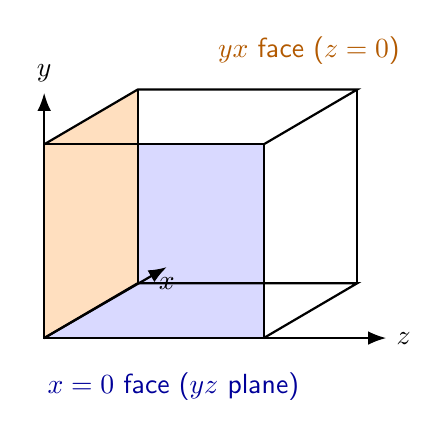
\begin{tikzpicture}[>=Latex,font=\sffamily,scale=0.82]
% 3-D cube: z is horizontal, y is vertical, x points down-right.
\coordinate (O) at (0,0);
\coordinate (Z) at (3.4,0);
\coordinate (Y) at (0,3.0);
\coordinate (X) at (1.45,0.85);
\coordinate (ZY) at (3.4,3.0);
\coordinate (ZX) at (4.85,0.85);
\coordinate (YX) at (1.45,3.85);
\coordinate (ZYX) at (4.85,3.85);
\fill[blue!15] (O)--(Z)--(ZY)--(Y)--cycle;
\fill[orange!25] (O)--(Y)--(YX)--(X)--cycle;
\draw[thick] (O)--(Z)--(ZY)--(Y)--cycle;
\draw[thick] (O)--(X)--(ZX)--(Z);
\draw[thick] (Y)--(YX)--(ZYX)--(ZY);
\draw[thick] (X)--(YX);
\draw[thick] (ZX)--(ZYX);
\draw[->,thick] (Z)--(5.3,0) node[right] {$z$};
\draw[->,thick] (O)--(0,3.8) node[above] {$y$};
\draw[->,thick] (O)--(1.9,1.1) node[below] {$x$};
\node[blue!60!black,align=left] at (2.0,-0.75) {$x=0$ face ($yz$ plane)};
\node[orange!70!black,align=left] at (4.1,4.45) {$yx$ face ($z=0$)};
\end{tikzpicture}
\end{document}
